\documentclass[12pt,a4paper]{amsart}
\usepackage[slovene]{babel}
\usepackage[utf8]{inputenc}
\usepackage{amsmath,amssymb,amsfonts}
\usepackage{url}
\usepackage[dvipsnames,usenames]{color}
\usepackage{graphicx}

\newcommand{\program}{FINANČNA MATEMATIKA}
\newcommand{\ime}{Brina Ribič, David Rozman}
\newcommand{\naslovdela}{Naključni sprehodi v lizikah}
\newcommand{\letnica}{2022}

\begin{document}
    
\begin{center}
    \thispagestyle{empty}
\noindent{\large
UNIVERZA V LJUBLJANI\\[1mm]
FAKULTETA ZA MATEMATIKO IN FIZIKO\\[5mm]
\program\ -- 1.~stopnja}
\vfill
\end{center}


\begin{center}
{\bf \naslovdela}\\[10mm]
Poročilo\\[1cm]
\end{center}
\vfill

\begin{center}
    Avtorja: {\large
\ime}\\[2mm]
   \noindent{\large
Ljubljana, \letnica} 
\end{center}
\pagebreak

\tableofcontents
\newpage

\section{Uvod}
V tem poročilu bova predstavila rezultate projektne naloge 'Naključni sprehodi v lizikah'. Najprej bova predstavila
problem ter kako sva se ga lotila, nato pa prikazala rezultate analize z grafi in tabelami.

\section{Opis problema}
Graf v obliki lizike je podan s parom $(m,n)$, kjer $m$ predstavlja število vozlišč polnega grafa, $n$ pa število
vozlišč na grafu poti. Da dobimo graf lizike, oba grafa povežemo z mostom. Po grafu opravimo naključni sprehod. V 
odvisnosti od parametrov $m$ in $n$ so naju zanimali sledeči pričakovani časi:
\begin{itemize}
    \item Pričakovani čas, da obiščemo vsa vozlišča v grafu (Čas pokritja)
    \item Pričakovani čas, da pridemo od enega v drugo vozlišče (Čas dosega)
    \item Pričakovani čas, da se vrnemo v začetno vozlišče (Čas vrnitve)
\end{itemize}
Zanimalo naju je tudi, kaj se zgodi s pričakovanim časom, če graf malce spremeniva, na primer dodava na drugi konec
poti še en poln graf itd.

\begin{figure}[h]
    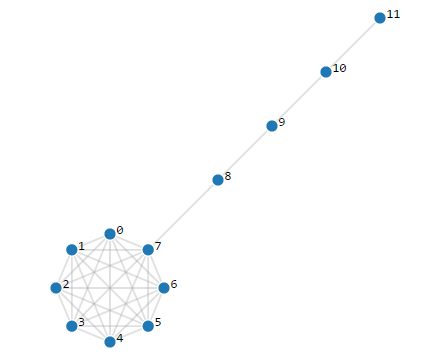
\includegraphics[width=\textwidth]{Lollipop_graph.png}
    \caption{Graf lizike (8,4)}
\end{figure}

\section{Potek reševanja}
Za reševanje problema sva uporabila programski jezik Python. Najprej sva napisala funkcije, ki zgenerirajo želeni graf.
Kot argument sprejmejo število vozlišč, vrnejo pa slovar, kjer ključi predstavljajo vozlišča, vrednosti so pa seznami
sosednjih vozlišč. Nato sva sestavila funkcije, ki po grafu opravijo naključni sprehod. Delujejo na sledeč način: 
Postavimo se v začetno vozlišče. Na vsakem koraku se premaknemo v naključno sosedno vozlišče, ki ga poberemo iz
seznama sosedov. Postopek ponavljamo dokler določen pogoj ni izpolnjen (npr. trenutno vozlišče je enako začetnemu,
če nas zanima čas vrnitve). Nazadnje sva definirala še funkcije, ki opravijo želeno število ponovitev naključnih sprehodov
in vrnejo povprečni čas.
Za vsak tip povprečnega časa, ki sva ga želela analizirati, sva naredila ustrezno veliko število ponovitev poskusov v
za več parametrov $m$ in $n$. Iz tabel in grafov sva nato poskusila ugotoviti časovno zahtevnost.

\section{Navaden graf lizike}

Najprej si bomo pogledali analizo navadnega grafa lizike, sestavljenega iz klike z $m$ vozlišči, poti z $n$ vozlišči in
mosta.

\subsection{Čas pokritja}

Da dobimo pravi čas pokritja, si moramo izbrati primerno začetno vozlišče. Z malo razmisleka hitro ugotovimo, da je
za najdaljši čas sprehoda po celotnem grafu potrebno začeti v vozlišču na kliki, ki ni del mostu, kajti tako, da bo
trajalo najdlje časa, da pridemo do konca poti, ki je najtežje dosegljivi del grafa.

Sledeča tabela prikazuje pričakovani čas pokritja glede na parametre $m$ in $n$. Za vsak primer sva izvedla 100.000
naključnih sprehodov in za pričakovani čas vzela njihovo povprečje.

\begin{table}[!ht]
    \centering
    \begin{tabular}{|l|l|l|l|l|l|l|l|l|l|}
    \hline
        m-n & 2 & 3 & 4 & 5 & 6 & 7 & 8 & 9 & 10 \\ \hline
        3 & 19 & 30 & 43 & 59 & 76 & 96 & 116 & 139 & 165 \\ \hline
        4 & 32 & 49 & 68 & 90 & 113 & 139 & 165 & 195 & 226 \\ \hline
        5 & 49 & 74 & 102 & 131 & 162 & 195 & 230 & 267 & 307 \\ \hline
        6 & 71 & 105 & 142 & 182 & 222 & 265 & 311 & 359 & 410 \\ \hline
        7 & 96 & 143 & 193 & 243 & 296 & 351 & 407 & 467 & 528 \\ \hline
        8 & 125 & 186 & 248 & 313 & 381 & 452 & 520 & 594 & 667 \\ \hline
        9 & 158 & 235 & 314 & 394 & 479 & 564 & 651 & 741 & 836 \\ \hline
        10 & 196 & 290 & 386 & 485 & 588 & 690 & 799 & 904 & 1009 \\ \hline
    \end{tabular}
\end{table}

Opazimo, da povečanje parametra $m$ bolj vpliva na pričakovani čas kot povečanje parametra $n$. To je zato, ker 
ima vsako vozlišče v kliki veliko povezav in traja veliko časa, da bomo obiskali vsa, medtem ko imamo na poti vedno
največ 2 izbiri za naslednje vozlišče.

Na naslednjih grafih vidimo kako povečanje določenega parametra vpliva na pričakovani čas. Prva trojica prikazuje
spreminjanje časa pri fiksnem $m$ in naraščajočim $n$, v drugi trojici pa sta vlogi zamenjani.

\begin{figure}[h]
    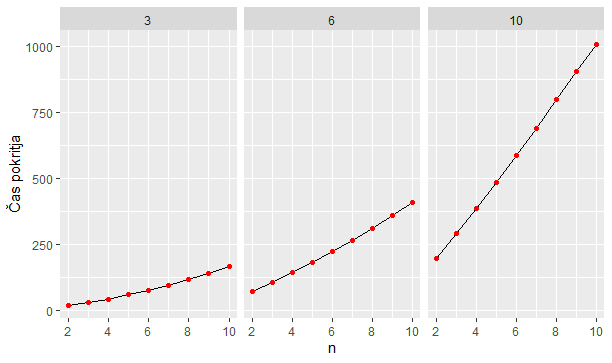
\includegraphics[width=\textwidth]{Rplot.png}
\end{figure}

\begin{figure}[h]
    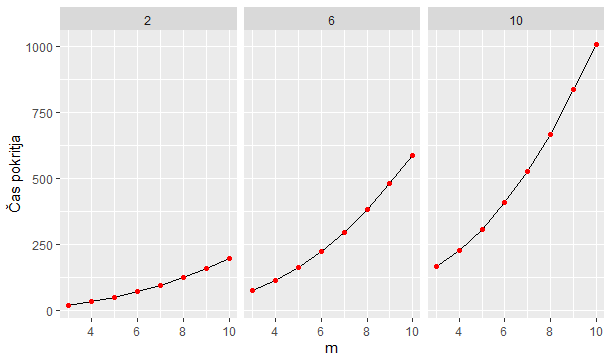
\includegraphics[width=\textwidth]{fiksenn.png}
\end{figure}

Vidimo, da se z $n$-jem pričakovani čas povečuje skoraj linearno, z $m$-jem pa rahlo kvadratično. Če si še ogledamo
vrednosti v tabeli, hitro opazimo, da je pričakovani čas pri nekem $m$ in $n$ vedno blizu $m^2n$. Tako smo pokazali,
da je pričakovani čas sprehoda po grafu lizike $\mathcal{O}(m^2n)$.

Tu bi poudarili še pomembnost začetne izbire vozlišča. Enak eksperiment sva izvedla še z začetkom v vozlišču na koncu
poti. Naslednja tabela prikazuje, kako se pričakovani čas pokritja spremeni, če si izberemo napačno začetno vozlišče.

\begin{table}[!ht]
    \centering
    \begin{tabular}{|l|l|l|l|l|l|l|l|l|l|}
    \hline
        m-n & 2 & 3 & 4 & 5 & 6 & 7 & 8 & 9 & 10 \\ \hline
        3 & 10 & 16 & 25 & 36 & 48 & 64 & 80 & 98 & 119 \\ \hline
        4 & 12 & 18 & 27 & 37 & 49 & 64 & 80 & 99 & 119 \\ \hline
        5 & 14 & 21 & 29 & 39 & 51 & 65 & 82 & 100 & 120 \\ \hline
        6 & 17 & 23 & 31 & 41 & 54 & 68 & 84 & 102 & 122 \\ \hline
        7 & 20 & 26 & 34 & 44 & 56 & 70 & 86 & 104 & 124 \\ \hline
        8 & 23 & 29 & 37 & 47 & 59 & 73 & 89 & 107 & 127 \\ \hline
        9 & 27 & 33 & 41 & 50 & 62 & 76 & 92 & 110 & 130 \\ \hline
        10 & 30 & 36 & 44 & 54 & 65 & 79 & 95 & 113 & 132 \\ \hline
    \end{tabular}
\end{table}

Ker smo začeli v težko dosegljivem vozlišču smo hitro prehodili celotno pot, ostala pa je le še klika, ki smo jo hitro
prehodili. Opazimo, da v tem primeru sprememba $m$ zelo malo vpliva na čas pokritja.




\end{document}
